\documentclass[review]{elsarticle}

\usepackage{amssymb,amsmath}
\usepackage{lineno}

\usepackage{xcolor}
\usepackage{bm}
\usepackage{mathrsfs}
\usepackage{dsfont}
\usepackage{graphicx, subfigure}	
%\usepackage{float}
\usepackage{algorithm}
%\usepackage[noend]{algpseudocode}
\usepackage{algpseudocode}

\biboptions{sort&compress}

\DeclareMathOperator*{\argmax}{arg\,max}

\journal{Neurocomputing}

\begin{document}
	
	\begin{frontmatter}
		
		\title{On two statistical models for simulating multi-label data}
		
		\author[UCL]{Miguel Valencia Garza}
		\ead{m.garza.12@ucl.ac.uk}
		\author[MEL]{Guoqi Qian}
		\ead{qguoqi@unimelb.edu.au}
		\author[UCL]{Jing-Hao Xue\corref{corr}}
		\ead{jinghao.xue@ucl.ac.uk}
		\cortext[corr]{Corresponding author. Tel.: +44-20-7679-1863; Fax: +44-20-3108-3105}
		\address[UCL]{Department of Statistical Science, University College London, London WC1E 6BT, UK}
		\address[MEL]{School of Mathematics and Statistics, The University of Melbourne, Parkville VIC 3010, Australia}
		
		\begin{abstract}
			In order to select an appropriate classifier it is important to know under which circumstances candidate classifiers will perform well or badly. A convincing and widely-accepted way to achieve this is through testing the classifiers on simulated data, where the ground truth is known and can be modified. However, in multi-label classification, few articles have focused on methods of simulating multi-label data. In this paper, we present a study and comparison of two popular statistical models which are capable of simulating multi-label data. We aim to provide insights on how the models' parameters affect three important multi-label attributes, namely label density, imbalance and unconditional dependence, of the simulated data. Our experiments suggest that the chain of logistic regressions model is a good choice to simulate data with moderate label dependence and imbalance, and the conditional logistic regression model is useful when high degrees of dependence and label imbalance are needed. 
		\end{abstract}
		
		\begin{keyword}
			Multi-label classification\sep data simulation\sep statistical models
		\end{keyword}
		
	\end{frontmatter}
	
	\linenumbers
	
	
	\section{Introduction}
	\label{INTRO}
	
	Even in the most mundane of classification tasks, one may assign an instance to more than one class; e.g., a specific person (in this case the instance) might be classified as neighbour, friend and classmate (from a set of possible classes), simultaneously. The task of assigning two or more classes (or labels) to an instance is known as multi-label classification~\citep{Tsoumakas:07, de2009tutorial, zhang2014review, Gibaja:15}. Multi-label classification has been widely utilised in practice, including very recent applications in bioinformatics, multimedia annotation, image categorisation, computer vision, and natural language understanding, to name a few~\citep{Tsoumakas:07, zhang2014review, meng2016plant, li2016conditional, hou2016multi, ivasic2016two, wu2015multi, zhao2015multi, zhao2015joint, yang2016exploiting, li2015supervised, li2015centroid}.
	
	In order to select the appropriate classifier for a given situation, it is useful to know the advantages and disadvantages of each candidate classifier. In particular, it is important to know under which circumstances the classifier will perform well and under which it will perform badly. A convincing and well-accepted way to achieve this is by testing the classifiers on simulated data, where we know the ground truth. 
	
	However, few articles have focused on methods of simulating multi-label data. The majority of papers use several benchmark real-world datasets to test the performance of their classifiers. Some researchers in multi-label learning have devised ad hoc methods to simulate multi-label data in order to test their methods.
	From our perspective, there are three main approaches to simulating multi-label data, namely geometry-based, rule-based and statistical model-based approaches.
	
	The geometry-based approach creates geometrical figures within a predefined space and populates them with $p$-dimensional points that correspond to the instances. Each geometrical figure represents a label and they are allowed to intersect. The subspace formed by these intersections translates into instances with multiple labels. For example, \citet{EG4} define a hyper-sphere with radius $r$ such that all instances are generated within. Then $q$ hyper-spheres with radii $r_{i} < r,$ $\forall i \in \{1,\ldots,q\}$, are randomly drawn inside the big hyper-sphere. These smaller hyper-spheres represent the labels and instances that are contained inside characterise them. Eventually, two or more hyper-spheres will share a subset of their instances, and this originates a multi-label setting.
	\citet{MLG2} follow a strategy similar to~\citep{EG4}, while~\citet{MLG1} is unlike from these two. \citet{MLG1} develop a multi-label data generator that conducts a heuristic search on a space of hypotheses in order to find one that splits the instances such that the dataset's characteristics are as close as possible to those specified by the user. The set of hypotheses consists of groups of hyperplanes that may define a linear or nonlinear classifier; the subspace in which two or more hyperplanes intersect determines the co-occurrence of multiple labels. 
	
	In the rule-based approach, the labels are assigned to an instance following a set of predefined rules, which can be deterministic or probabilistic. Usually, a small subset of labels, say $m < q$ (where $q$ is the total number of labels), is generated by some stochastic mechanism. Then, these $m$ labels create the rest $q-m$ ones by following the rules of co-occurrence. For instance, in~\cite{EG3} two simple rules are employed to simulate multi-label data: label $j$ is relevant when label $i$ is relevant; or label $i$ and label $j$ cannot be relevant/irrelevant at the same time. These two rules give way to variants of them that can be applied as well. For this example, it is only necessary to generate label $i$ since label $j$ is controlled by the state of $i$; this process ensures dependence between pairs of labels.
	
	In the statistical model-based approach, the data-generating process is conducted via a statistical model. By modifying the model's parameters, different characteristics can be elicited on the datasets generated. \citet{EG2} simulate a multi-label dataset that consists of two predictors and three labels. The predictors are generated using a mixture of Gaussians model; each component of the mixture represents a different combination of the labels. This is, every combination of labels is treated as a category and then each category is allocated to one component of the mixture.
	\citet{EG1} simulate various multi-label datasets on a set of linear models for the $q$ labels with corresponding values $y_j$, for $j = 1,\ldots,q$, as
	\begin{displaymath}
	y_{j} = h_{j}\left( \mathbf{x} \right) + \epsilon_{j} \left( \mathbf{x} \right),
	\end{displaymath} 
	in which they call $h_{j}$ the structural part and $\epsilon_{j}$ the stochastic part of the model. They induce different degrees of label dependences by varying the structural and stochastic parts of the models, respectively. Higher similarity among the parameters of the model, i.e.~the structural part, increases the degree of unconditional dependence; when the stochastic parts of the statistical models are equal ($\epsilon_{1}(\mathbf{x}) = \ldots = \epsilon_{q}(\mathbf{x})$), labels are conditionally dependent. 
	
	Opting for any of the aforementioned three approaches has advantages and disadvantages. For instance, the geometry-based approach can be thought as a `general' simulation method, since it rarely describes a specific real process, such as assigning several tags to a chunk of text. On the other hand, a rule-based method may resemble this tagging process with higher fidelity. Moreover, the rules may be able to exclude cases that are impossible or illogical to occur. However, the downside of it is that it may be too specific.
	Statistical models help characterise the reality whilst accounting for its inherent variability, under certain simplifying assumptions. That is, a statistical model-based approach can help simulate a real process under a controlled environment with its uncertainty taken into account, providing an appealing middle ground between a too general approach and a too specific one. 
	
	In this context, this paper presents a comparison of two popular statistical models which are capable of simulating multi-label data. Our contribution is on investigating and demonstrating the similitudes and differences in characteristics that these models induce in the generated datasets, in terms of label dependence, density and imbalance. In particular, we seek to provide insights on how the models' parameters affect these multi-label attributes. Ultimately, these aspects will depict a profile of each model and provide with useful information for practitioners in generating and using simulated multi-label data.
	
	
	\section{Models for simulating multi-label data}
	\label{MODELS}
	
	We shall give a brief overview of the two statistical models and explain how to use them to simulate multi-label data.  In order to exemplify them, we resort to the following notation: $n$ is the sample size or number of instances, $p$ is the number of predictors, and $q$ is the number of labels.
	
	\subsection{Models}\label{ss:models}
	
	A typical multi-label dataset of $n$ instances can be expressed in terms of an $n\times p$ matrix consisting of $n$ observed data vectors of $p$ predictors, with each vector of predictors denoted by $\mathbf{x} \in \Re^{p}$, and an $n\times q$ matrix consisting of $n$ vectors of $q$ assigned labels, with each vector of labels denoted by $\mathbf{y} \in \{ 0,1 \}^{q}$. This is, the multivariate distribution $p(\mathbf{x},\mathbf{y})$ is defined for a set of mixed variables including both continuous and discrete variables.
	
	There are various statistical models able to handle mixed variables. Among these models, we chose those that characterise the conditional distribution $p(\mathbf{y}|\mathbf{x})$, since this distribution allows us to explicitly model label conditional dependence. %is aligned with a discriminative strategy for classification.
	The two statistical models chosen to generate synthetic multi-label data for the experiments and comparisons are the following:
	\begin{enumerate}[(i)]
		\item Chain logistic regression for dependent binary variables. This model has been used for simulating multi-label datasets by~\citet{PCC}.
		\item Conditional logistic regressions model. To the best of our knowledge, this model has not been used to generate multi-label data.
	\end{enumerate}
	
	\subsubsection{Chain logistic regressions for dependent binary variables}
	
	Originally proposed by~\citet{CHAIN}, this model characterises the conditional distribution $p(\mathbf{y}\mid\mathbf{x})$ by factorising it into a product of $q$ probabilities as
	%%
	\begin{equation} \label{CC}
	p(\mathbf{y}\mid\mathbf{x}) = p(y_{1}\mid\mathbf{x})\, p(y_{2}\mid\mathbf{x}, y_{1}) \cdots p(y_{q}\mid\mathbf{x}, y_{1},\ldots, y_{q-1})\ ,
	\end{equation}
	where $\mathbf{y}=\left(y_{1},\ldots,y_{q} \right)^T$ as before.
	If each factor of (\ref{CC}) is defined as a logistic regression, then the computational and analytical tools available for univariate logistic regression can be used for the set of dependent variables. Fitting this model is then equivalent to fitting $q$ independent logistic regression models, each with an incremental set of predictors:
	\begin{eqnarray}
	f_{j} \left( P(y_{j} = 1 \mid y_{1},\ldots,y_{j-1},\mathbf{x}) \right) &=& \log \left[ \frac{P(y_{j} = 1\mid y_{1},\ldots,y_{j-1},\mathbf{x})}{P(y_{1} = 0\mid y_{1},\ldots,y_{j-1},\mathbf{x})} \right] \nonumber\\
	&=& \mathbf{x}^T \bm{\beta}_j + \gamma_{j1} y_{1} + \ldots + \gamma_{j,j-1} y_{j-1}\ ,
	\label{eq:cc}
	\end{eqnarray}
	where $\bm{\beta}_{j}$ is the vector of coefficients (including one for the intercept with $\mathbf{x}$ augmented if necessary) for predictors $\mathbf{x}$, and $\gamma_{ji}$, for $i<j$, is the parameter that controls the dependence between $y_{j}$ and its predecessors $y_{i}$. 
	
	An advantageous feature of this model is that its decomposition is intuitive, since it follows from the product rule of probability. However, in the context of multi-label learning the order of the labels affects the testing/prediction phase. For example, in (\ref{CC}) we need to predict $y_{1}$ before we predict $y_{2}$, and then use these two estimates to predict $y_{3}$, and so on.
	
	\citet{OCC} and~\citet{PCC} confirmed this order-prediction issue when they applied (\ref{CC}) to different multi-label datasets. As a way to overcome this drawback, they propose to use an ensemble of chain classifiers (as they rename this model) in which each component of the ensemble uses a different ordering. For data simulation, the ordering represents another parameter which we can impose arbitrarily.
	
	\subsubsection{Conditional logistic regressions}
	
	The conditional logistic regressions model was first proposed by~\citet{JOE} and then revisited by~\citet{MVB}. It models $p(\mathbf{y}|\mathbf{x})$ based upon a set of compatible conditional logistic regression models (one for each element of $\mathbf{y}$), since a well-established framework exists for (univariate) logistic regression. That is, the conditional distribution of $y_{j}$ given the rest of the variables is modelled by a logistic regression; for example, when $q=2$,
	%%
	\begin{eqnarray*}
		f_1 \left( P(y_{1} = 1 \mid y_{2},\mathbf{x}) \right) &=& \log \left[ \frac{P(y_{1} = 1\mid y_{2},\mathbf{x})}{P(y_{1} = 0\mid y_{2},\mathbf{x})} \right] = \mathbf{x}^T\bm{\beta} _{1} + \theta_{12}y_{2}\ , \\
		f_2 \left( P(y_{2} = 1 \mid y_{1},\mathbf{x}) \right) &=& \log \left[ \frac{P(y_{2} = 1\mid y_{1},\mathbf{x})}{P(y_{2} = 0\mid y_{1},\mathbf{x})} \right] = \mathbf{x}^T\bm{\beta} _{2} + \theta_{21}y_{1}\ ,
	\end{eqnarray*}
	%%
	where $\bm{\beta}_{i}$ is the vector of coefficients for predictors $\mathbf{x}$, and $\theta_{ij}$ is the parameter that controls the dependence between $y_{i}$ and $y_{j}$. A necessary and sufficient condition for these logistic regressions to be compatible is that $\theta_{12} = \theta_{21}$~\citep{JOE}. Thus, the joint (conditional) distribution is given by
	%%
	\begin{equation} \label{JC}
	p(y_{1},y_{2}|\mathbf{x}) = \frac{1}{c(\mathbf{x})} \exp \left \{ \sum^{2}_{i=1}{y_{i} \left( \mathbf{x}^T \bm{\beta}_{i} \right)} + \sum_{1 \leq i < j \leq 2}{y_{i}y_{j}\theta_{ij}} \right\}\ ,
	\end{equation}
	%%
	where $c(\mathbf{x}) = 1 + \exp(\mathbf{x}^T\bm{\beta}_{1}) + \exp(\mathbf{x}^T\bm{\beta}_{2}) + \exp(\mathbf{x}^T\bm{\beta}_{1}+\mathbf{x}^T\bm{\beta}_{2} + \theta_{12})$ is the constant of normalisation.
	
	For any $q$, the generalisation is straightforward, and it holds that the necessary and sufficient condition for compatibility is that $\theta_{ij} = \theta_{ji}$. For larger dimensions of $\mathbf{y}$, the dependence structure can be extended to higher-order interactions among predictors-labels and/or labels-labels.
	
	\subsection{Implementations}
	
	For the chain of logistic regressions model, in Algorithm~\ref{CHLa} we simulate labels one at a time, augmenting the predictor space with the previous ones until we reach the last one.
	%%
	\begin{algorithm}[H]
		\caption{Chain of logistic regressions model}\label{CHLa}
		\begin{algorithmic}[1]
			\State{Generate a vector of $p$ independent continuous predictors; e.g. $\mathbf{x} \sim \mathscr{N}_{p}(\mathbf{0},\mathbf{I})$}
			\State{${y}_{1} \sim \mathrm{Bernoulli}(p_{1})$, where $p_{1} = \left(1 + \exp(-\mathbf{x}^T \bm{\beta}_{1}) \right)^{-1}$}
			\For{$j = 2$ to $q$}
			\State{Augment predictor space $\mathbf{x}_{a} = \left( \mathbf{x},{y}_{1},\ldots,{y}_{j-1} \right)^T$}
			\State{Augment coefficient vector $\bm{\beta}_{a} = \left(\bm{\beta}_{j},\gamma_{j,1},\ldots,\gamma_{j, j-1} \right)^T$}
			\State{${y}_{j} \sim \mathrm{Bernoulli}(p_{j})$, where $p_{j} = \left(1 + \exp(-\mathbf{x}^{T}_{a} \bm{\beta}_{a}) \right)^{-1}$}
			\EndFor
		\end{algorithmic}
	\end{algorithm}
	
	In Algorithm~\ref{CNDa} we take advantage of the conditional formulation of the model and use a Gibbs-sampling-like procedure to draw samples. The downside of this process is that Algorithm~\ref{CNDa} is the more time-consuming.
	%%
	\begin{algorithm}[H]
		\caption{Conditional logistic regressions model}\label{CNDa}
		\begin{algorithmic}[1]
			\State{Generate a vector of $p$ independent continuous predictors; e.g. $\mathbf{x} \sim \mathscr{N}_{p}(\mathbf{0},\mathbf{I})$}
			\State{Assign arbitrary values to labels; e.g. $\mathbf{y}^{(0)} \sim \mathrm{Bernoulli}(0.5)$}
			\Repeat
			\State{Sample from the $q$ conditional logistic regressions (one for each label)}
			\Until{reach a predetermined number of iterations.}
		\end{algorithmic}
	\end{algorithm}
	
	
	\section{Label dependence, density and imbalance of multi-label datasets}\label{s:attributes}
	
	We aim to compare the selected statistical models' ability to control the attributes of the simulated multi-label data, in particular to elicit different degrees of dependence among the labels, which is one of the most important attributes to depict the data. We expect that an increase/decrease in the unconditional dependence among labels will also affect other multi-label data attributes, such as label density (and cardinality) and label imbalance.
	
	\subsection{Label dependence}
	
	Given that an instance may belong to more than one class simultaneously, one of the most important assumptions supporting a multi-label classifier is with regard to the dependence among labels. According to~\citet{EG1}, there are two kinds of label dependence that can be acknowledged in the multi-label framework, namely
	%%
	\begin{description}
		\item[\it Unconditional dependence] This type of dependence exists solely within the labels. A random vector of labels $\mathbf{y} = \left(y_{1},\ldots,y_{q} \right)$ is unconditionally independent if
		\begin{equation} \label{UDEP}
		p(\mathbf{y}) = \prod^{q}_{j=1}{p(y_{j})}\ .
		\end{equation}
		\item[\it Conditional dependence] This type of dependence describes the relationship among the labels given a specific instance $\mathbf{x}$. A random vector of labels $\mathbf{y} = \left(y_{1},\ldots,y_{q} \right)$ is conditionally independent given $\mathbf{x}$ if
		\begin{equation} \label{CDEP}
		p(\mathbf{y}\mid\mathbf{x}) = \prod^{q}_{j=1}{p(y_{j}\mid\mathbf{x})}\ .
		\end{equation}
	\end{description}
	
	The two statistical models that we investigate here are defined such that $p(\mathbf{y}\mid\mathbf{x}) \neq \prod^{q}_{j=1}{p(y_{j}\mid\mathbf{x})}$, which means that labels generated by these models are conditionally dependent. The degree of label conditional dependency is given by the models' parameters. We try different values of the parameters (including zero, which implies label conditional independence) to elicit various degrees of conditional dependency but we do not measure it since it is given in the models' definition.
	
	To measure unconditional dependence, we can resort to traditional methods for measuring dependence among discrete random variables such as $G$-test or $\chi^{2}$-test. In this case, we choose to measure it using a measure of multivariate dependence from information theory called total correlation~\citep{refTC1,refTC2,refTC3}. We measure label unconditional dependence as  
	%the method proposed by~\citet{MLG1} and defined as
	%%
	%\begin{equation}
	%Udep(\mathbf{y}) = \frac{\sum_{i < j}\{\rho \left( {y}_{i}, {y}_{j} \right) \cdot | {y}_{i} \cap {y}_{j} |\}}{\sum_{i < j}{| {y}_{i} \cap {y}_{j} |}}\ ,
	%\end{equation}
	%where $\rho(\cdot)$ is the correlation coefficient between ${y}_{i}$ and ${y}_{j}$ in absolute value and $| {y}_{i} \cap {y}_{j} |$ is the number of instances in which $y_{i}$ and $y_{j}$ are both equal to 1. The advantage of using this metric is that it allows to assign a numeric value to the unconditional dependence, and its value is 0 when labels are unconditionally independent and 1 when they are all equal (maximum dependence).
	
	\begin{equation}\label{TC}
	Udep(\mathbf{y}) = \frac{\sum^{q}_{j=1}{ \{ H(y_{j}) \} - H(y_{1},\ldots,y_{q})}}{\sum^{q}_{j=1}{ \{ H(y_{j}) \} - \max_{y_{j}} \{H(y_{j})\} }}
	\end{equation}
	
	where $H(y_{j})$ is the information entropy of label $y_{j}$, $H(y_{1},\ldots,y_{q})$ is the joint entropy of the label set and $\max_{y_{j}} \{H(y_{j})\}$ is the highest entropy value in the label set. The numerator in (\ref{TC}) is the definition of total correlation. 
	
	Since $\max \{ H(y_{1}),\ldots,H(y_{q}) \} \leq H(y_{1},\ldots,y_{q})$ with equality when all variables are deterministic functions of one of the variables, the denominator in (\ref{TC}) represents the maximum value of total correlation that can be attained by a set of labels. We use this quotient to keep the value of label unconditional dependence in $[0,1]$, where 0 represents unconditional independence and 1 labels that are highly dependent.
	
	\subsection{Label cardinality \& density}
	
	Another multi-label data attribute often monitored is cardinality. This attribute refers to the number of active labels per instance in a multi-label dataset. More specifically, \emph{label cardinality} is the average number of active labels per instance~\citep{Tsoumakas:07,Gibaja:15}, calculated as
	%%
	\begin{equation}
	Cardinality = \frac{1}{n} \sum^{n}_{i=1}{\left(\sum^{q}_{j=1}{\mathds{1}\left[y_{ij} = 1 \right]}\right)}\ ,
	\end{equation}
	where the indicator function $\mathds{1}[\cdot]$ takes value 1 when the argument inside the brackets is true and 0 otherwise, and $y_{ij}$ is the value of the $j$th label of the $i$th instance.
	
	Label cardinality is an important measure since it also gives a rough idea about the order dependency among the labels (e.g. pairwise, three-way, etc.); which will eventually help in the selection of a good classification strategy.
	
	A related metric for this type of label distribution is \emph{label density}~\citep{Tsoumakas:07,Gibaja:15}, which is defined as
	%%
	\begin{equation}
	L.Density = \frac{Cardinality}{q}\ .
	\end{equation}
	
	For two or more datasets with an equal number (denoted by $q$) of labels, comparing their label distributions can be done using either their $Cardinality$ or $L.Density$ indices. This is, both metrics convey the same message about the distribution of relevant labels among datasets. However, datasets with different number of labels can only be compared via their $L.Density$ indices. In this paper, we report $L.Density$ as a measure of label distribution.
	
	\subsection{Label imbalance}
	
	In a multi-label setting, it is likely that a label, say the $j$th label, does not appear often or, on the contrary, appears quite frequently. This entails a poor representation of such label since not many examples contain it (or is over-represented). Then the classifier will be prone to errors since it would be difficult to predict correctly when label $j$ occurs in an unseen example. This problem is called \emph{label imbalance}.
	
	In \emph{single-label} classification, the issue of imbalance refers to the case that a class (from the disjoint set of possible classes) is represented by much fewer instances than another class. This generalises from one to multiple labels. This is, we say that there is label imbalance when a label is highly underrepresented or overrepresented. Different authors have generated different ways to measure label imbalance of a dataset. \citet{LIEG1} take the ratio between the maximum and minimum numbers of ones or zeros per label, and use the mean value of the ratios as the dataset's imbalance index. \citet{LIEG2} make a more elaborate ratio. They take the maximum count of ones among the labels and divide it by the count of ones for each label, such that the label with the higher count of ones (highest imbalance) will have index equal to one and the rest will have indices greater than one.  \citet{LIEG3} resort to entropy as measure of label imbalance. However, these measures have no clear bounds or need an extra metric to perform comparisons among datasets.
	
	To overcome this issue, we devise an index to help measure the degree of label imbalance in a dataset. Our imbalance index measures the ratio of ones and zeros that a label contains. For instance, for label $j$ we count how many ones and zeros it has and compute $count_{j}(1)/count_{j}(0)$. We take $\log_{10}$ of these counts so we have
	%%
	\begin{eqnarray} \nonumber
	L.Imbalance_{j} &=& \log_{10}(count_{j}(1) + \mathds{1}[count_{j}(1) = 0]) \\  &-& \log_{10}(count_{j}(0) + \mathds{1}[count_{j}(0) = 0])\ .
	\end{eqnarray}
	In this way, we can have a magnitude and sign of label $j$'s imbalance; e.g.~if there are more zeros than ones, then we will have a \emph{negative} value. It is clear that the index is defined in the range $-\log_{10}(n) \leq L.Imbalance_{j} \leq \log_{10}(n)$. 
	
	Finally, we compute the \emph{root mean square} (RMS) value of $L.Imbalance_{j}$, for $j=1,\ldots,q$, as a metric of dataset's imbalance; i.e.
	%%
	\begin{equation}\label{LIMB}
	L.Imbalance_{\mathbf{y}} = \sqrt{\frac{1}{q} \sum^{q}_{j=1}{\left( L.Imbalance_{j} \right)^{2} }}\ .
	\end{equation}
	A larger value of $L.Imbalance_{\mathbf{y}}$ implies a higher degree of label imbalance in the dataset. For our experiments, we are able to compare indices because $n$ is the same for all generated data. For comparison between datasets with different $n$ values, we suggest to replace $L.Imbalance_{\mathbf{y}}$ by $L.Imbalance_{\mathbf{y}}/\log_{10}(n)$ and perform comparisons based on the latter metric. The range of $L.Imbalance_{\mathbf{y}}/\log_{10}(n)$ is always $[0,1]$, enabling standardised comparison.
	
	
	\section{Experimental studies}
	
	\subsection{Experimental setup \& questions for investigation}
	\label{DEXPER} 
	
	Here we set up experiments to monitor the changes in attributes (presented in section~\ref{s:attributes}) of simulated multi-label datasets, which are induced by the two statistical models described in section~\ref{ss:models}.
	
	The experiments consist of models generating synthetic multi-label datasets across different values of their parameters and dimensions. To take account of the variability of the data generated, we replicated the data-generating process 100 times. We divided the experiments in two parts. In the first part, we fixed the number of labels $q=3$ and vary the number of predictors, $p = \{ 3, 6, 12, 24\}$. For the second one, we fixed the number of predictors $p = 2$ (plus an intercept term) and vary the number of labels, $q = \{ 3, 6,12, 24\}$. For both parts, we assign the parameters five different values to achieve different degrees of conditional dependence. These parameters are defined as follows:
	%%
	\begin{itemize}
		\item Chain of logistic regressions model: $\gamma_{{j}i} = \gamma \in \{ -10, -5, 0, 5, 10 \}$ for function $f_{j}$ such that
		\begin{equation}\label{eq:param:gamma}
		f_{j} = \mathbf{x}^T\bm{\beta}_{j} + \gamma \sum_{i=1}^{j-1} y_{i}\ .
		\end{equation}
		\item Conditional logistic regressions model: $\theta_{ji} = \theta \in \{ -10, -5, 0, 5, 10\}$ for function $f_{j}$ such that
		\begin{equation}\label{eq:param:theta}
		f_{j} = \mathbf{x}^T \bm{\beta}_{j} + \theta \sum^{q}_{i \neq j}{y_{i}}\ .
		\end{equation}
	\end{itemize}
	
	Although the setting is simple, it suffices to help us discover and illustrate the patterns emerging in data's characteristics for the following three scenarios that are of common interest to practitioners in multi-label classification.
	%%
	\begin{enumerate}[(a)]
		\item \emph{What if the models' parameters controlling the dependence between labels are changed?} 
		\item  \emph{What if the number of predictors $p$ increases?} 
		\item \emph{What if the number of labels $q$ increases?} 
	\end{enumerate}
	
	
	\subsection{Results and discussion}
	
	We implemented the experiments in statistical software \texttt{R}~\citep{RR}. We report the mean values and standard deviation of label imbalance, density, unconditional dependence and conditional dependence.
		
		\subsubsection{Label dependence}
		
		\begin{figure}[H]
			\begin{center}
				\subfigure[Varying $\gamma$, $\theta$ \& $p$]{%
					\label{fig:results:dep:ud:p}
					\includegraphics[width=0.49\textwidth]{ud_p.pdf}
				}%
				\subfigure[Varying $\gamma$, $\theta$ \& $q$]{%
					\label{fig:results:dep:ud:q}
					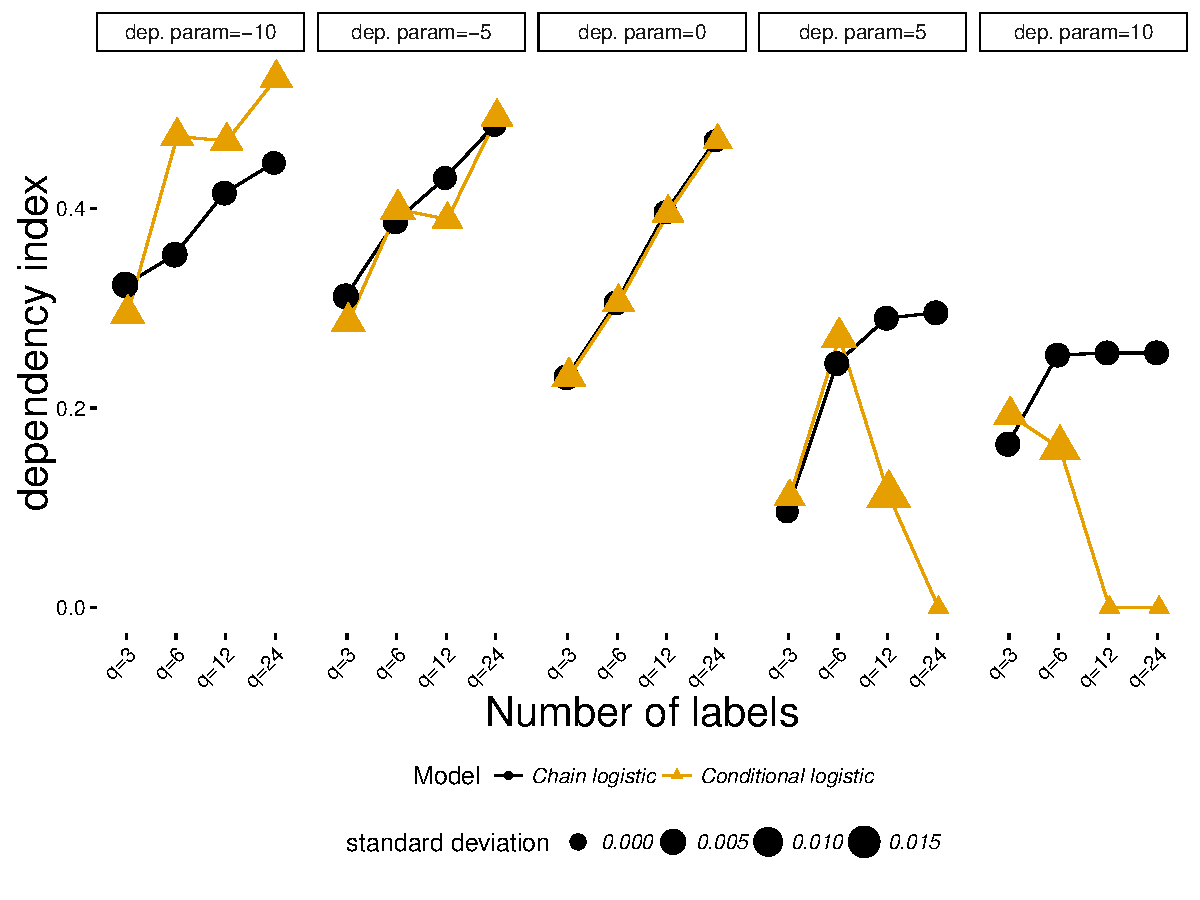
\includegraphics[width=0.49\textwidth]{ud_q.pdf}
				}%
			\end{center}
			\caption{Unconditional dependence. The plots show the change in dependency index as we vary the number of predictors $p$, the number of labels $q$ and the value of the parameters controlling the dependency amongst labels $\gamma$ and $\theta$ (denoted as \emph{dep. param} in the plot).}
			\label{fig:results:dep}
		\end{figure}
		
		We can observe from Figure~\ref{fig:results:dep} the following:
		
		\emph{Change in $\gamma,\theta$}. We observe two patterns: for varying number of predictors, increasing the values of the parameters controlling the dependence among labels increases unconditional dependence. When we vary the number of labels it seems that unconditional dependence decreases. For either varying the number of predictors or the number of labels, we expected an increase in dependence as we increased the absolute value of $\gamma$ and $\theta$, depicting a $U$-shape pattern when we vary $\gamma, \theta$ from -10 to 10. We discuss the reason of a different pattern when changing the value of $q$ below, when we comment about varying the number of labels.
		
		As aforementioned, for varying $p$ we see a monotonic-like increase in unconditional dependence. The departure from the expected pattern is likely caused by the values of \textbf{X} and $\bm{\beta}_{1}, \bm{\beta}_{2}$ and $\bm{\beta}_{3}$ that help labels to achieve a higher degree of unconditional dependence for large positive values of $\gamma$ and $\theta$.
		
		%The dependency index that we chose assigns importance to co-occurrence of ones. This is, it gives more importance to pairs of labels that are one at the same time. This indicates that for negative values of $\gamma$ and $\theta$, $P(y_{j}=1) < P(y_{j}=0)$ whilst for $0 \leq \gamma, \theta$ it happens the opposite situation: $P(y_{j}=1) > P(y_{j}=0)$. 
		
		%For this particular setting it seems that the difference on magnitude of these probabilities is larger for positive values of $\gamma$ and $\theta$ than for negative ones. This leads to assign importance to more pairs of labels, depicting the increasing pattern that we observe.
		
		\emph{Change in $p$}. As we increase the number of predictors the unconditional dependence decreases as well with no apparent increase in variability. We expected this behaviour because as we increase the number of predictors, with fixed number of labels, the strength of the dependence among labels relies more and more on the predictors. Since all predictors have different parameter $\bm{\beta}_{j}, j \in \{ 1,2,3 \}$ it is also expected that the generated labels become more different to each other as the predictors' importance increases. If all $\bm{\beta}_{j}, j \in \{ 1,2,3 \}$ were the same we would see an increasing pattern in unconditional dependence as $p$ grows because labels would become more and more similar to each other.
		
		\emph{Change in $q$}. The unconditional dependence increases as the number of labels increases. This increase in dependence was expected because the importance of the labels' parameters grows with the number of labels. Since $\gamma$ and $\theta$ take the same value for all labels the similarity amongst labels tends to increase. 
		
		For $\gamma, \theta > 0$ we observe an anomaly with conditional logistic regressions model as the number of labels grows. The data suggests that for positive values of $\theta$, the marginal distribution of the labels generated by conditional logistic regressions model behave like $P(y_{j}=1) > P(y_{j}=0)$. As we increase the number of labels (and $\theta > 0$) the difference between these probabilities increases as well. In fact, $P(y_{j}=1)$ grew so much that there were labels that took only values of one. This translates in zero variability or, equivalently, zero entropy which is what we see in Figure \ref{fig:results:dep:ud:q}. The same effect takes place in chain of logistic regression's simulated data but in less degree, which makes it unable to depict the $U$-pattern that we expected when varying $\gamma$ from -10 to 10.
		
		The experiments suggest that conditional logistic regressions model attains higher degrees of unconditional dependence than chain of logistic regressions model. Although, for large value of labels and large positive value of $\theta$ we need to proceed with caution because conditional logistic regressions model is prone to generate labels that take only one value, which causes a serious decrease in unconditional dependence. Then, if high degree of unconditional dependence is needed and we have many labels (more than ten) it is better to use chain of logistic regressions model. Otherwise, conditional logistic regressions model is a suitable model to simulate multi-label datasets with high label unconditional dependence.
		
		\subsubsection{Label imbalance}
		
		\begin{figure}[H]
			\begin{center}
				\subfigure[Varying $\gamma$, $\theta$ \& $p$]{
					\label{fig:results:imb:p}
					\includegraphics[width=0.49\textwidth]{li_p.pdf}
				}%
				\subfigure[Varying $\gamma$, $\theta$ \& $q$]{
					\label{fig:results:imb:q}
					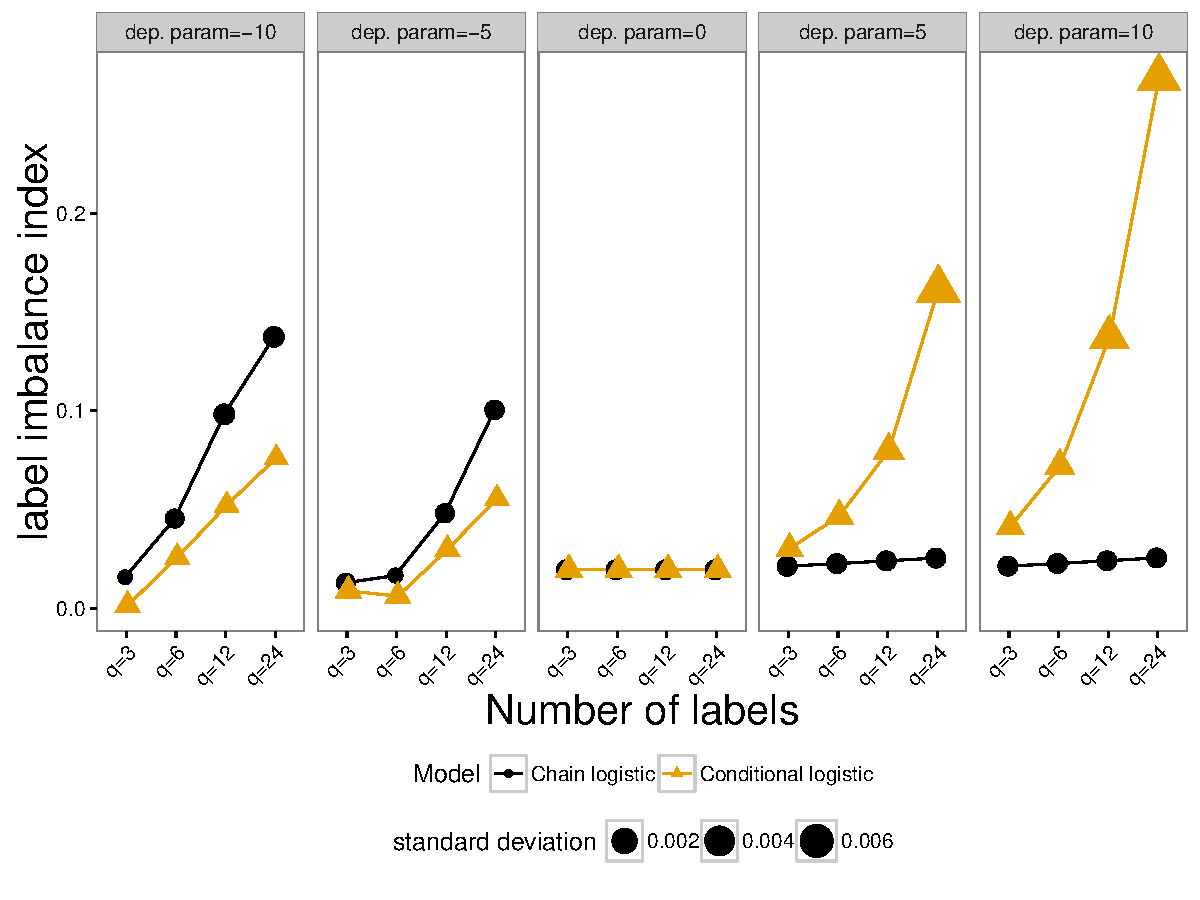
\includegraphics[width=0.49\textwidth]{li_q.pdf}
				}
			\end{center}
			\caption{Label imbalance. The plots show the change in mean label imbalance index (or the RMS of the individual label imbalance indices) as we vary the number of predictors $p$, the number of labels $q$ and the value of the parameters controlling the dependency between labels $\gamma$ and $\theta$ (denoted as \emph{dep. param} in the plot).}
			\label{fig:results:imb}
		\end{figure}
		
		The plots for the label imbalance index, measured from the datasets simulated by the two statistical models, is shown in Figure~\ref{fig:results:imb}, from which we can make the following observations.
		
		\emph{Change in $\gamma,\theta$}. We appreciate an increase in label imbalance as we increase the absolute value of parameters $\gamma$ and $\theta$. In other words, we observe a $U$-shaped pattern as we vary $\gamma$ and $\theta$ from their more negative value to their more positive value. 
		
		We expected such behaviour as these parameters can be seen as $P(y_{j}=1|\mathbf{x},\mathbf{y}_{\mathrm{subset}})$'s conditional log-odds ratio. Then, an increase or decrease in the value of $\gamma, \theta$ affects the ratio ones/zeros appearing in a label. We observe that positive values of $\gamma$ and $\theta$ affect more the ratio ones/zeroes (i.e.~creates greater imbalance) than negative values.
		
		\emph{Change in $p$}. We see that the maximum value of imbalance is achieved when we got six predictors. More than six predictors decreases label imbalance. This particular pattern corresponds to the specific values taken by \textbf{X},  $\bm{\beta}_{1}, \bm{\beta}_{2}$ and $\bm{\beta}_{3}$. In general, we expect that as we increase the number of predictors the importance of $\gamma$ and $\theta$ reduces, making the ratio ones/zeros more balanced.
		
		\emph{Change in $q$}. We observe that an increase in the number of labels increases the label imbalance index. We expected this behaviour because we know that, for both models, the labels are generated by $p(y_{j}|\mathbf{x},\mathbf{y}_{\mathrm{subset}})$. This means that adding more labels affects the probability of $y_{j}=1$, which increases the number of ones (or zeroes) appearing in each label.
		
		We observe again, from another perspective, the effect of large positive $\theta$ and large number of labels interaction in the conditional logistic regressions model. As we mentioned above, we get higher imbalance measurements than those from chain logistic regressions model.
		
		\subsubsection{Label density}
		
		\begin{figure}[H]
			\begin{center}
				\subfigure[Varying $\gamma$, $\theta$ \& $p$]{
					\label{fig:results:density:p}
					\includegraphics[width=0.49\textwidth]{ld_p.pdf}
				}%
				\subfigure[Varying $\gamma$, $\theta$ \& $q$]{
					\label{fig:results:density:q}
					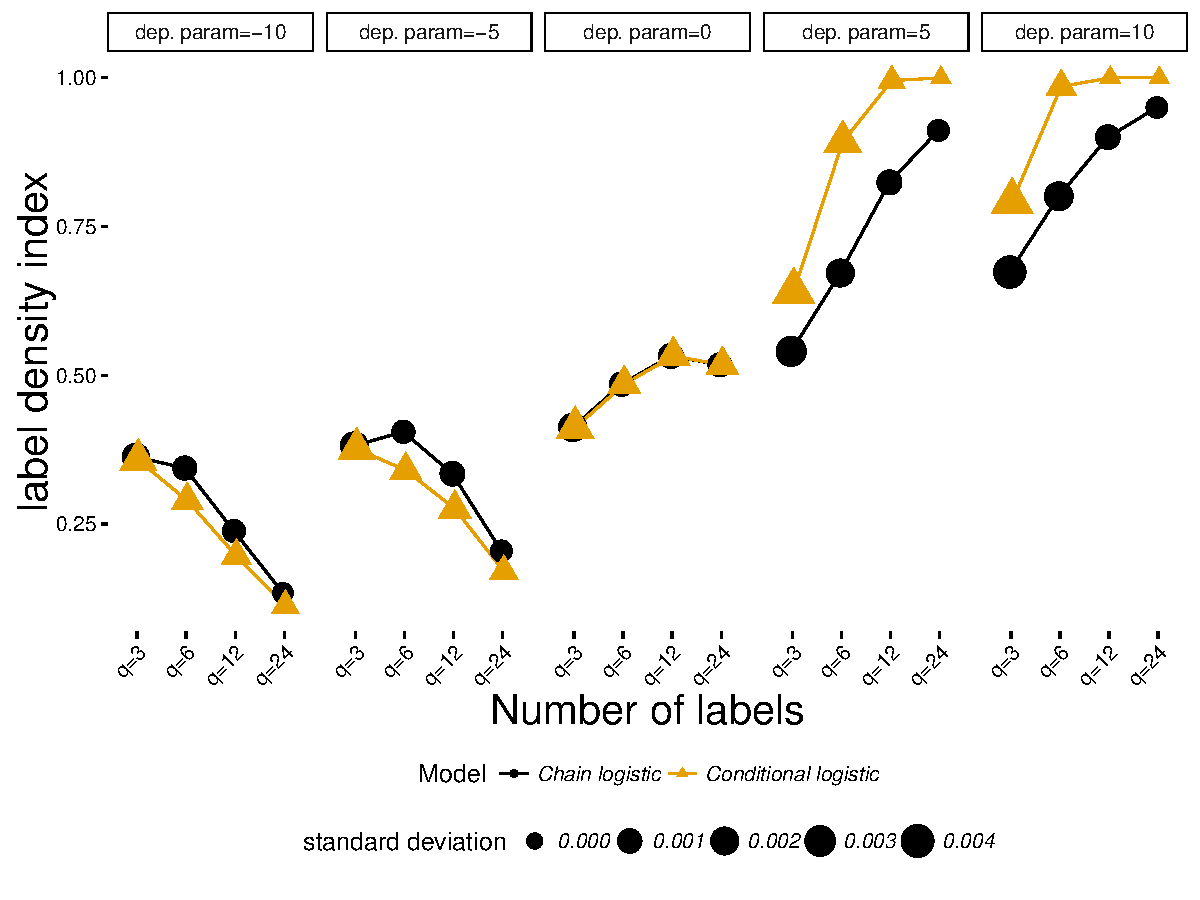
\includegraphics[width=0.49\textwidth]{ld_q.pdf}
				}
			\end{center}
			\caption{Label density. The plots show the change in label density as we vary the number of predictors $p$, number of labels $q$ and the value of the parameters controlling the dependency between labels $\gamma$ and $\theta$ (denoted as \emph{dep. param} in the plot).}
			\label{fig:results:density}
		\end{figure}
		
		From Figure~\ref{fig:results:density}, we can make three observations.
		
		\emph{Change in $\gamma,\theta$}. There is an increase in label density as the values of $\gamma$ and $\theta$ grow. We expected this increasing pattern since label density counts the number of ones in an instance. 
		
		As we have seen, negative values of $\gamma, \theta$ increase the probability of $y_{j}=0$, which gives less ones per instance. When we increase the value of $\gamma, \theta$, the probability of $y_{j}=1$ increases as well. This makes label density more likely to be greater for positive values of $\gamma, \theta$ than for negative ones.
		
		\emph{Change in $p$}. We observe that increasing the number of predictors makes the label density decrease. This is because higher number of predictors reduces the importance of $\gamma$ and $\theta$, which are the parameters that link label with label. Less influence of $\gamma, \theta$ makes co-occurrences of ones less likely. 
		
		\emph{Change in $q$}. Increasing the number of labels generates two patterns that need to be observed jointly with the values of $\gamma$ and $\theta$. For negative values of $\gamma, \theta$, label density decreases as the number of labels increases. For $0 \leq \gamma, \theta$ as the number of labels increases, label density increases as well. Again, this has to do with the fact that we are counting ones.
		
		Since larger (and positive) values of $\gamma, \theta$ increase the probability of $y_{j}=1$, increasing the number of labels boosts this probability, generating the growing pattern that we observe in the plots. An analogue situation occurs for negative values of $\gamma$ and $\theta$. The low probability of $y_{j}=1$ for these values in addition to an increase in number of labels brings this probability down.
		
		Finally, we observe larger values of density from the conditional logistic regressions model due to the effect of large positive $\theta$ and large number of labels interaction that we discussed above.
		
		\section{Conclusion}
		\label{CONCL} %Limitations of the study, scope. Focus on statistical models. No generalisation. Give possible reasons (with arguments) about the results of experiments. Are there new unexpected results/patterns?
		
		In this paper we conducted several experiments aiming to discover the patterns elicited in multi-label attributes when data were generated by two statistical models, namely chain of logistic regressions and conditional logistic regressions. We commented about how to measure synthetic data's multi-label attributes. 
		
		The conditional logistic regressions model renders the highest increase of the attributes measured when its dependence parameter $\theta$ is increased,  for fixed number of predictors and labels. Using the experiments' simple dependency setting, this model is useful when high degrees of unconditional dependence, cardinality and label imbalance are required. If the user wants high unconditional dependence, it is important to monitor label imbalance to avoid unwanted issues related with it. On the other hand, if for some reason the user needs high label imbalance then this model is the most useful choice between the two models.
		
		The chain of logistic regressions model reacts less aggresively than the conditional logistic regressions model to changes in its dependence parameter $\gamma$. This makes the model useful for simulating data with dependent labels and moderate label imbalance and cardinality. It allows the user to increase the value of $\gamma$ more than conditional logistic regressions' $\theta$, without quickly falling in problems of label imbalance. It is important to remind the reader that, for multi-label learning, the order in which labels are generated matters for the chain of logistic regressions model. Thus, it is important to keep record of label ordering and/or treat it as an extra parameter.
		
		
		\section*{Acknowledgements}
		M. Valencia Garza gratefully acknowledges a scholarship from Consejo Nacional de Ciencia y Tecnologia (CONACyT).
		
		\section*{References}
		
		\bibliographystyle{elsarticle-num-names}
		\bibliography{MLC-simulation}
		
	\end{document}
	
	\endinput
